\newpage
\section{WS2812 Ansteuerung \- Entwicklung des Aserial Moduls (Aufgabe 7)}

\subsection{Implementierung des Aserial Moduls}

Um die korrekte Ansteuerung der WS2812 zu gewährleisten, werden die genauen Taktzeiten für die High und Low Phasen berechnet. 

Da die 50 MHz Clock genutzt wird, beträgt die Periode 20 ns.


$$T=\frac{1}{50 MHz} = 20 ns$$

Eine Dauer von 900 ns bzw. 350 ns entspricht demnach folgenden Taktzeiten:
\[
\text{Takte für } 900\,\mathrm{ns}
= \frac{900\,\mathrm{ns}}{20\,\mathrm{ns}}
= 45\,\text{Takte}
\]

\[
\text{Takte für } 350\,\mathrm{ns}
= \frac{350\,\mathrm{ns}}{20\,\mathrm{ns}}
= 17.5\,\text{Takte}
\]

Der Taktzyklus von 17.5 wird auf 18 Perioden aufgerundet.

Ein ganzes Bit dauert theoretisch 1.25 µs, was 62.5 Takten entspricht. Diese Bitzeit wird auf 63 Takte aufgerundet.
Grundsätzlich kann eine Ungenauigkeit von 150 ns bzw. 7.5 Taktzyklen toleriert werden.

\inputminted[linenos,frame=single,fontsize=\footnotesize]{vhdl}{A7_Abgabe/testbench_ws2812/ws2812_aserial.vhd}

Der VHDL Code implementiert das Aserial Modul, welches die WS2812 LEDs entsprechend der berechneten Taktzeiten ansteuert.
Erst nach 350 ns wird das anliegende, zu sendende Bit gelesen um sicherzustellen, dass es aufgrund verzögerter Signale nicht zu Fehlinterpretationen kommt.

\subsection{Testbench für das Aserial Modul}

\inputminted[linenos,frame=single,fontsize=\footnotesize]{vhdl}{A7_Abgabe/testbench_ws2812/tb_ws2812.vhd}

Die Testbench simuliert die Ansteuerung der WS2812 LEDs indem sie eine Bitfolge von 1010 in MSB-First Reihenfolge sendet.
Alle, an das DUT (Device Under Test) angelegten Signale werden in der Testbench definiert und gesteuert, um die Funktionalität des Aserial Moduls zu überprüfen.

\subsection{Simulationsergebnisse}

\begin{figure}[H]
\centering
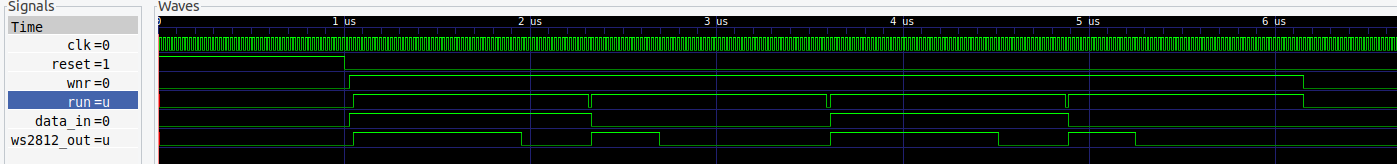
\includegraphics[width=\textwidth]{A7_Abgabe/resources/ganzeSimulation.png}
\caption{Simulation des Aserial Moduls. Die Bitfolge 1010 wird in MSB-First Reihenfolge gesendet.}
\label{fig:Aserial Simulation}
\end{figure}

In der Simulation ist zu erkennen, dass die Bitfolge 1010 korrekt gesendet wird. 

Im Folgenden werden die einzelnen Bits genauer betrachtet, um die Einhaltung der Timing-Anforderungen zu überprüfen. Hierfür wurden Marker gesetzt,
um die Taktflangen zu messen. 

\begin{figure}[H]
\centering
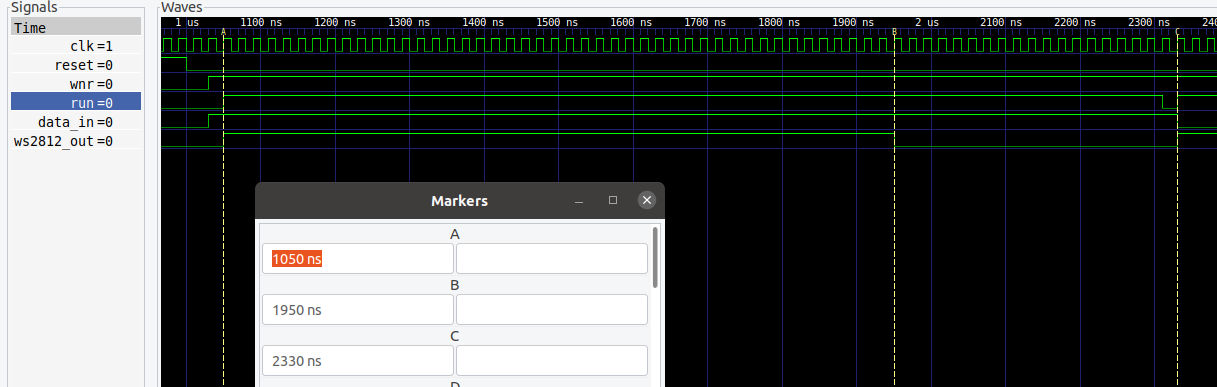
\includegraphics[width=\textwidth]{A7_Abgabe/resources/eins.png}
\caption{Timing des ersten Bits}
\label{fig:Erstes Bit mit Markern}
\end{figure}                                                          

Aus den Markern ergeben sich Zwischenzeiten von 360 ns und 920 ns, was innerhalb der tolerierbaren Ungenauigkeit liegt.

\begin{figure}[H]
\centering
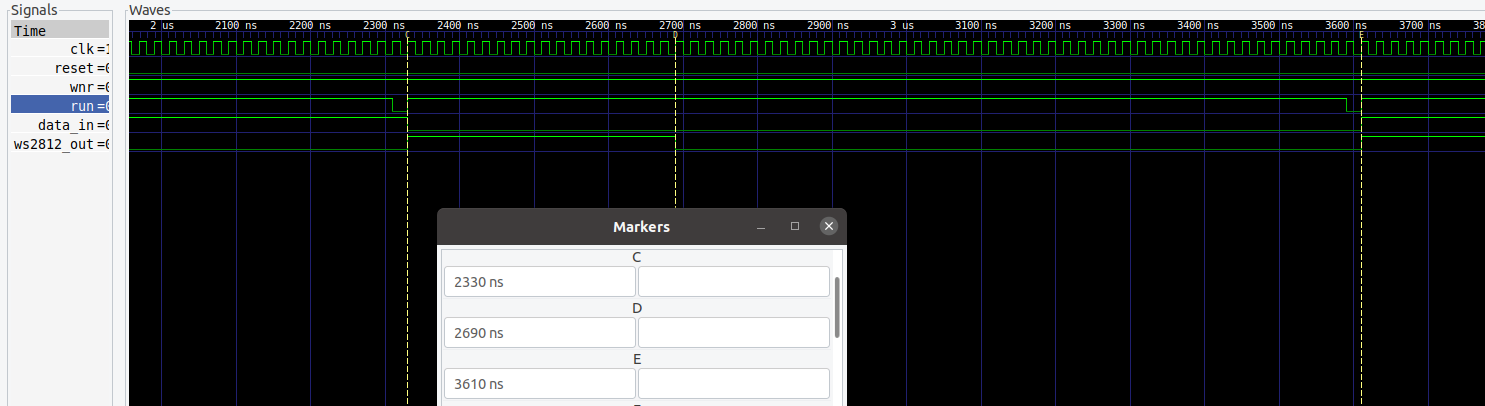
\includegraphics[width=\textwidth]{A7_Abgabe/resources/zwei.png}
\caption{Timing des zweiten Bits}
\label{fig:Zweites Bit mit Markern}
\end{figure}

Aus den Markern ergeben sich Zwischenzeiten von 900 ns und 380 ns, was innerhalb der tolerierbaren Ungenauigkeit liegt.


\begin{figure}[H]
\centering
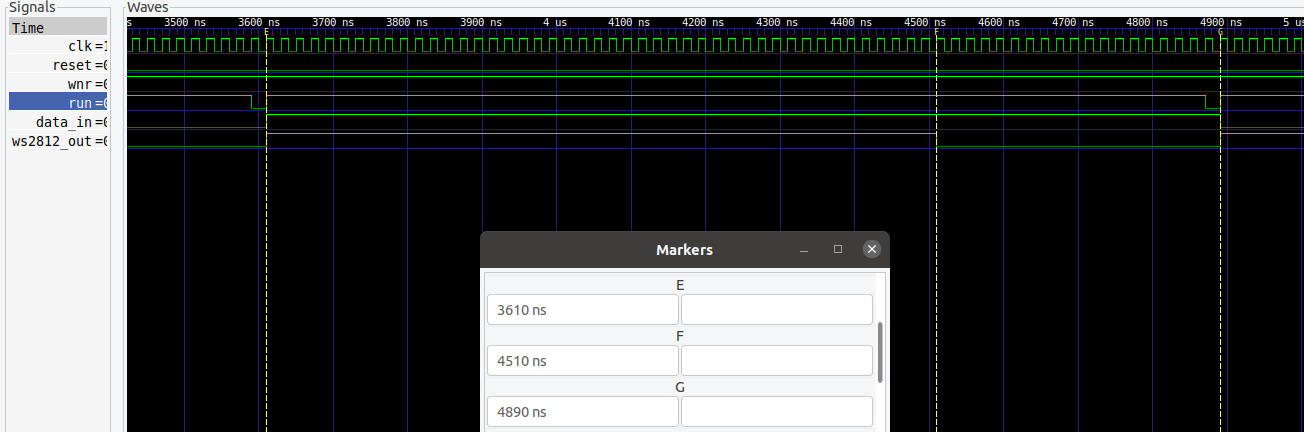
\includegraphics[width=\textwidth]{A7_Abgabe/resources/drei.png}
\caption{Timing des dritten Bits}
\label{fig:Drittes Bit mit Markern}
\end{figure}

Aus den Markern ergeben sich Zwischenzeiten von 900 ns und 380 ns, was innerhalb der tolerierbaren Ungenauigkeit liegt.


\begin{figure}[H]
\centering
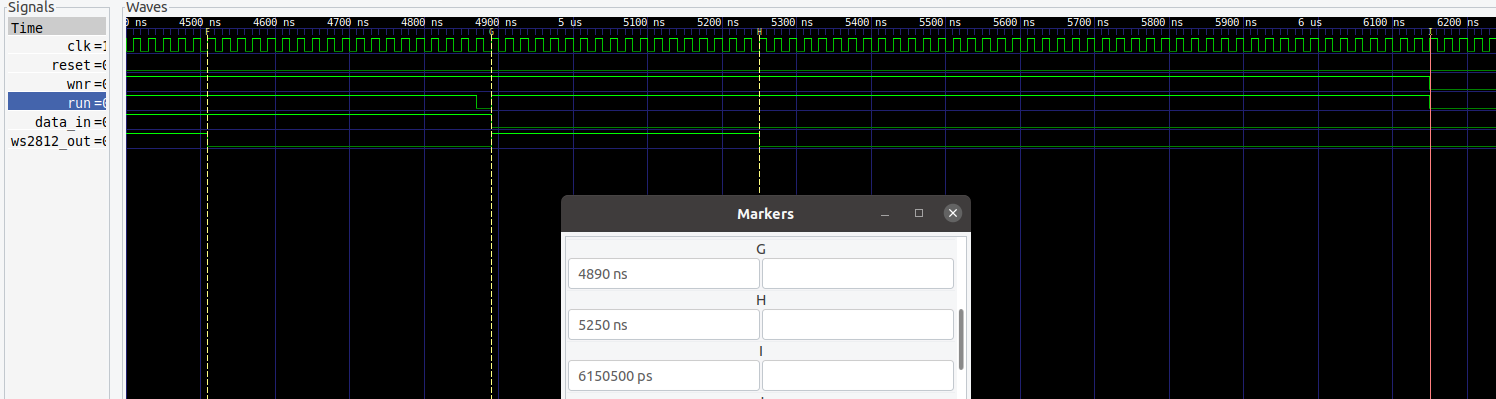
\includegraphics[width=\textwidth]{A7_Abgabe/resources/vier.png}
\caption{Timing des vierten Bits}
\label{fig:Viertes Bit mit Markern}
\end{figure}

Aus den Markern ergeben sich Zwischenzeiten von 360 ns und 900.5 ns, was innerhalb der tolerierbaren Ungenauigkeit liegt.
